% The research corpus (ci/research.json): newtx (Times-like text and
% mathematics), pgfplots, algorithmicx, cleveref, subcaption.
\documentclass[10pt,twocolumn]{article}
\usepackage[T1]{fontenc}
\usepackage{newtxtext,newtxmath}
\usepackage{amsmath}
\usepackage{booktabs}
\usepackage{pgfplots}
\pgfplotsset{compat=1.18}
\usepackage{algorithm}
\usepackage{algpseudocode}
\usepackage{subcaption}
\usepackage[hidelinks]{hyperref}
\usepackage{cleveref}
\title{Scaling Laws for Toy Models}
\author{C. Author \and D. Author}
\date{}
\begin{document}
\maketitle
\begin{abstract}
A two-column paper in newtx with plots drawn by pgfplots and pseudocode
by algorithmicx, as machine-learning and systems papers are written.
\end{abstract}
\section{Introduction}
We follow the literature~\cite{shannon1948,knuth1984}. \Cref{fig:loss}
shows the loss; \cref{alg:train} gives the loop and \cref{tab:hp} its
settings. Mathematics in newtx: $\mathcal{L}(\theta) = \frac{1}{N}
\sum_{i=1}^{N} \ell(f_\theta(x_i), y_i) + \lambda \lVert\theta\rVert_2^2$,
with $\alpha, \beta, \Gamma, \Omega \in \mathbb{R}$.

\begin{figure}[t]
\centering
\begin{subfigure}{\columnwidth}
\centering
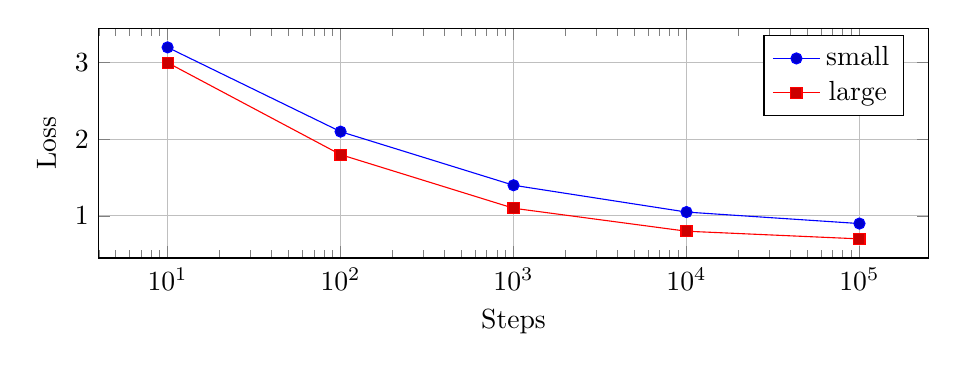
\begin{tikzpicture}
\begin{axis}[width=\columnwidth,height=4.5cm,xmode=log,xlabel={Steps},ylabel={Loss},
  legend pos=north east,grid=major]
\addplot+[mark=*] coordinates {(10,3.2) (100,2.1) (1000,1.4) (10000,1.05) (100000,0.9)};
\addplot+[mark=square*] coordinates {(10,3.0) (100,1.8) (1000,1.1) (10000,0.8) (100000,0.7)};
\legend{small,large}
\end{axis}
\end{tikzpicture}
\caption{Training loss.}\label{fig:loss-a}
\end{subfigure}
\begin{subfigure}{\columnwidth}
\centering
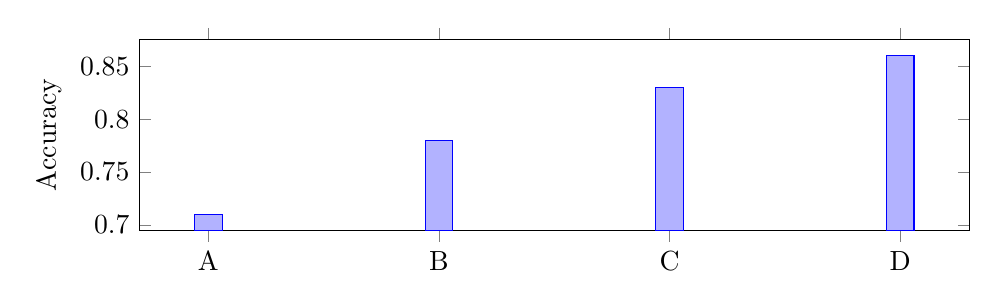
\begin{tikzpicture}
\begin{axis}[width=\columnwidth,height=4cm,ybar,symbolic x coords={A,B,C,D},xtick=data,ylabel={Accuracy}]
\addplot coordinates {(A,0.71) (B,0.78) (C,0.83) (D,0.86)};
\end{axis}
\end{tikzpicture}
\caption{Accuracy by model.}\label{fig:loss-b}
\end{subfigure}
\caption{Results.}\label{fig:loss}
\end{figure}

\begin{algorithm}[t]
\caption{Training loop}\label{alg:train}
\begin{algorithmic}[1]
\Require data $D$, learning rate $\eta$
\For{$t \gets 1$ \textbf{to} $T$}
  \State sample a batch $B \subset D$
  \State $\theta \gets \theta - \eta \nabla_\theta \mathcal{L}_B(\theta)$
  \If{converged}
    \State \textbf{break}
  \EndIf
\EndFor
\State \Return $\theta$
\end{algorithmic}
\end{algorithm}

\begin{table}[t]
\centering
\caption{Hyper-parameters.}\label{tab:hp}
\begin{tabular}{lrr}
\toprule
Parameter & Small & Large \\
\midrule
Layers & 6 & 24 \\
Width & 512 & 2048 \\
Learning rate & $3\times10^{-4}$ & $1\times10^{-4}$ \\
\bottomrule
\end{tabular}
\end{table}

\section{Discussion}
Larger models reach lower loss~\cite{lamport1994}, as \cref{fig:loss-a}
shows; \cref{fig:loss-b} agrees.

\bibliographystyle{plain}
\bibliography{refs}
\end{document}
